\documentclass[12pt]{article}
\usepackage[margin=1in]{geometry} 
\usepackage{amsmath,amsthm,amssymb,amsfonts}
\usepackage{setspace}
\doublespacing

\usepackage{tikz}
\usetikzlibrary{arrows,positioning,calc}
\newcommand\LM{\ensuremath{\mathit{LM}}}
\newcommand\IS{\ensuremath{\mathit{IS}}}

\tikzset{
    %Define standard arrow tip
    >=stealth',
    %Define style for boxes
    punkt/.style={
           rectangle,
           rounded corners,
           draw=black, very thick,
           text width=6.5em,
           minimum height=2em,
           text centered},
    % Define arrow style
    pil/.style={
           <-,
           thick,
           shorten <=2pt,
           shorten >=2pt,},
    % Node for explanation       
    punk/.style={
           rectangle,
           draw=white, thin,
           text width=17em,
           minimum height=2em,
           text centered}   
}


\begin{document}
 
\section{Introduction}

\section{Experimental Design and Procedures}
\subsection{Sample}
We collected data from 12 middle schools in Daegu, the fourth largest city in Korea in coordination with the Education Office. 4 classes from grade 1 in each school and additional 4 classes from grade 2 in 4 schools were selected for the classroom experiment\footnote{Basically, we chose classes at random. However, in case of coed schools which divide classes into all-boys and all-girls, we made the number of chosen classes from each case  equal.}. In total, 1610 students (64 classes) participated in the survey, composing much larger sample than in general lab experiments. And this enables us to study the variation of individual and collective decisions and the association between the two. Out of 1610 subjects, 1572 individuals (786 pairs) conducted both individual and collective decision treatment; many classes were odd-numbered so some subjects could not be paired.

Unlike former experimental studies on group decision which recruited couples (Abdellaoui et al. (2010), Bateman and Munro (2005), Palma et al. (2011)) or strangers (Baillon et al. (2016), Bone et al. (1999), Cason et al. (1997), Charness et al. (2007), Deck et al. (2012)), we constructed pairs within a classroom at random, which gives two important benefits. First, due to the random matching, we can exclude the effect of hidden factors for the matching process. Secondly, by matching classmates, we can help subjects to feel the experimental environment of making a decision together to be natural.  

In case of couples, even though it is common for them to do a group decision, it encompasses a lot of unobservable characteristics. They have been matched by themselves and developed their own way to reach a consensus. These hinder us from identifying the effect of properties of individual decision from that of other unobservable characteristics on group decision. We can handle it by recruiting subjects who don't know each other. However, it might be awkward for one to interact with a stranger. Also, this even does not represent the general group decision making process in our real life in that we usually cooperate someone whom we are acquainted with or at least have ice breaking time when we do with a stranger. 

\subsection{Design}
The decision environment is based on Choi et al. (2007). A subject confronts a sequence of decision problem under the risk and each problem is presented as a choice on a given budget line. In this setting, there are two states-state 1 and 2, and one is chosen randomly and equally likely. A subject chooses $(x_1,x_2)$ on the given budget line $p_1x_1+p_2x_2=1$ without knowing which state is realized, but only knowing that (s)he is paid off $x_1$ if the state is 1 and $x_2$ in the other case. In other words, the decision problem is equivalent to allocating the resource to two Arrow securities for state 1 and 2 given prices of assets $(p_1,p_2)$.
	
Figure 1 gives an example of our decision environment. If one chooses $A$ on the $45^\circ$ line, (s)he can equalize payoff in each state, perfectly hedging the risk at the expense of high return. On the other hand, choosing $C$ means one puts all the money to the cheaper goods, $x_1$, in this graphical illustration. Of course, it is possible to choose less extreme choices between $A$ and $C$, for instance, $B$. 

\begin{figure}[ht]
\caption{An Example of the Decision Problem}
\begin{center}
\begin{tikzpicture}[
        scale=1.2,
        IS/.style={black, thick},
        LM/.style={black, dashed},
        axis/.style={thick, ->, >=stealth', line join=miter},
        every node/.style={color=black},
        dot/.style={circle,fill=black,minimum size=4pt,inner sep=0pt,
            outer sep=-1pt},
    ]
    % axis
    \draw[axis,<->] (7,0) node(xline)[right] {$x_1$} -|
                    (0,5) node(yline)[above] {$x_2$};
    \draw[LM] (0,0) coordinate (LM_1) -- (4,4) coordinate (LM_2) node[above] {$x_1=x_2$};
    \draw[IS] (0,3) coordinate (IS_1) -- (6,0) coordinate (IS_2) ;
    %Intersection is calculated "manually" since Tikz does not offer
    %intersection calculation for parabolas
    \node[dot,label=above:$A$] at (2,2) (int1) {};
	\node[dot,label=right:$B$] at (4,1) (int1) {};
	\node[dot,label=above:$C$] at (6,0) (int1) {};		
\end{tikzpicture}
\end{center}
\end{figure}

\subsection{Procedures}
We conducted the experiment in all 64 classes for 8 days through the third and the fourth week in August, 2016. We recruited four experimenters to implement the experiment at the same time for the same grade from the same school\footnote{By doing so, we could control the spill-over effect within the same grade.}. We opened one session for each class and ran morning and afternoon sessions to cover 8 classes a day. In addition, to keep sessions from being significantly different depending on experimenters we gave them a one-day training and a clear guideline.

Each session lasted 100 minutes including a short break. At the first half, subjects participated 4 economic games including the decision making games\footnote{The other two were dictator and public good game combined with friendship network, which would be studied in another research.}. Then we had 10 minutes break. And the latter half was a sequence of friendship survey, 5 math questions and a non-cognitive survey.

All process was computerized using an on-line platform, O-tree (http://www.otree.org/). We set up laptops for every one of students and portable WIFI routers in the classroom. One technician per class was staying throughout a session to cope with any mechanical problems instantly. 
  
The decision making experiment was done at the end of the first half of each session. Basically, we have the within-subject design. To begin with, subjects made 18 rounds of individual decisions, which is described closely in the section 2.2. Each round started with computer's choosing intercepts on axes $x_1$ and $x_2$ (price of securities), between 300 (KRW) and 3000 (KRW), ensuring at least one of the intercepts is greater than or equal to 1500 (KRW). A subject could move the mouse cursor on the given budget line and a small box next to the cursor showed the exact value of coordination. Then one could pick a consumption bundle by clicking any favorable point (continuous choice set). After the 18 times of individual decisions, subjects were matched to pairs within a class and one of the two partners moved seat toward the other; matching partners and selecting movers were determined randomly. Pairs had 1 and half minutes of discussion time and made 18 times of decisions together. We did not give any direction on the way of making consensus and free conversation was allowed. And no feedback was given during the session\footnote{We make the sequence of first-individual-then-collective decision holds for all subjects. First reason is somewhat practical. To go through all experiments given the time limit, this order is beneficial because putting things back after the collective decision takes quite long. We also considered that keeping subjects calm after the group decision, which includes free conversation, might be tough. Secondly, as comparison between individual and collective decision was not our main interest, we did not take the order effect seriously. In fact, we find some differences between characteristics of the two but these might result from the learning by introspection (Note that the learning from feedback is not likely to be exist as there is no feedback). Therefore, we would not put much emphasis on these findings.}.

After all choices, one from individual choices and another one out of collective ones were randomly selected and the computer realized the states for each decision to determine the payoff. In particular, the payoff from collective choice was doubled and divided equally to both subjects, which makes partners' monetary gain be perfectly correlated. We sent the total payoff from all games so subjects could not decompose gains from each game. In addition, for educational purpose, the reimbursement was made in electric money which can be used in every 9,468 chain stores of the biggest convenience store company in Korea. 

\section{Rationality Extension}
Our first question is about the association of individual rationality and collective one. In the revealed preference approach, rationality is equated with the consistency within choices. Having different decision making ability and preference, individuals within a group have to compromise and reach a consensus to make consistent collective choices. 

In fact, there is a no clear logical relationship between the two. Rational individuals have well-defined preferences in their mind. They could find a way to the consensus more easily due to those clear images or make a conflict when those are controversial. 

\subsection{Testing Rationality}
We take the revealed preference approach to measure the rationality. In this approach, a set of choices is rational if it is consistent within a well-defined (complete and transitive) preference ordering. It is widely known that solutions for maximization of a non-satiated utility function are rational in this sense (REFERENCE). 

Many studies have taken this approach in testing rationality of individual choices (REFERENCE). We use the same way in testing the collective rationality, which is also in line with the representative agent model, a classical view on group decision in economics. It assumes even agents differ, they act in such a way that their collective choices are equivalent to the decision of one individual or many identical individuals. 

Due to Afriat (1967), which shows the equivalence between the existence of well-behaving (concave, continuous, and strictly increasing) utility function and data's satisfying Generalized Axiom of Revealed Preference (GARP) when the number of budget sets is finite, testing the rationality reduces to testing GARP. Denoting $X^t$ a chosen consumption given price $p^t$, $t=1,...,T$, GARP requires if $X^t$ is revealed preferred to $X^s$ then $X^s$ should not be strictly revealed preferred to $X^t$. In other words, if $p^t X^t \geq p^t X^s$, then $p^s X^t \geq p^s X^s$. 

However, GARP test has a limitation as an "all or nothing" notion: it only gives information on whether the data satisfy the test or not. As many of observation data have some violations of the theory, one may want to discriminate the severity of the inconsistency. This is why we need a measure on the degrees of how much the choices being close to passing GARP. 

There have been several attempts, but we use a well-known index proposed by Afriat (1972) \footnote{Appendix includes all the results of this section using Varian (1991)'s rather than Afriat (1972)'s CCEI.}. Critical Cost Efficiency Index (CCEI) is the largest number $e \in [0,1]$ such that $e p^{k1} X^{k1} \geq p^{k1} X^{k2}, e p^{k2} X^{k2} \geq p^{k2} X^{k3}, ..., e p^{kt-1} X^{kt-1} \geq p^{kt-1} X^{kt},...,e p^{kT-1} X^{kT-1} \geq p^{kT-1} X^{kT}, tk\in[1,2,...,T]$ implies $e p^{kT} X^{k1} \geq p^{kT} X^{kT}$. $e=1$ means there is no cycle in this preference relation without any adjustment to the budget sets. On the other hand, $e=0$ means this preference passes GARP only after getting rid of all the budget sets. Any numbers between 0 and 1 have a meaning between the two, with bigger ones corresponding to less adjustment to the budget set to rationalize the choice data. In other words, the higher the CCEI is, the more rational a choice data is.    

Figure 2 gives an graphical illustration of CCEI with only 2 data points. In this example, $X^t$ is chosen when $X^s$ is cheaper given price $p^t$, which implies $X^t$ is strictly revealed preferred to $X^s$. However, $X^s$ is also strictly revealed preferred to $X^t$ given $p^s$, leading to the violation of GARP. We can remove this violation by shifting the given budget line $p^tX^t$ to $e_tp^tX^t$ or $p^sX^s$ to $e_sp^sX^s$. In this case, CCEI equals to $e_t$ as this adjustment is minimal to attain consistency within choices.

\begin{figure}[ht]
\caption{A graphical illustration of CCEI}
\begin{center}
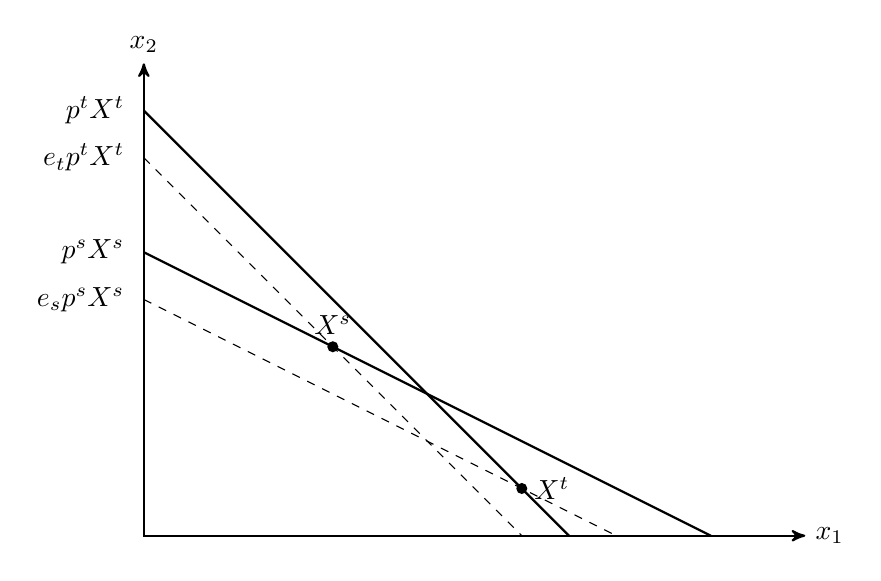
\begin{tikzpicture}[
        scale=1.2,
        IS/.style={black, thick},
        LM/.style={black, dashed},
        axis/.style={thick, ->, >=stealth', line join=miter},
        every node/.style={color=black},
        dot/.style={circle,fill=black,minimum size=4pt,inner sep=0pt,
            outer sep=-1pt},
    ]
    % axis
    \draw[axis,<->] (7,0) node(xline)[right] {$x_1$} -|
                    (0,5) node(yline)[above] {$x_2$};
    \draw[LM] (0,2.5) coordinate (LM_1) -- (5,0) coordinate (LM_2);
    \draw[LM] (0,4) coordinate (LM_1) -- (4,0) coordinate (LM_2);
    
    \draw[IS] (0,3) coordinate (IS_1) -- (6,0) coordinate (IS_2) ;
    \draw[IS] (0,4.5) coordinate (IS_1) -- (4.5,0) coordinate (IS_2) ;
    %Intersection is calculated "manually" since Tikz does not offer
    %intersection calculation for parabolas
    \node[label=left:$p^tX^t$] at (0,4.5) (int1) {};
    \node[label=left:$e_tp^tX^t$] at (0,4) (int1) {};
    \node[label=left:$p^sX^s$] at (0,3) (int1) {};
    \node[label=left:$e_sp^sX^s$] at (0,2.5) (int1) {};

    
    \node[dot,label=above:$X^s$] at (2,2) (int1) {};
	\node[dot,label=right:$X^t$] at (4,0.5) (int1) {};
\end{tikzpicture}
\end{center}
\end{figure}


\subsection{Collective Rationality}

\begin{center}
-Figure 3 here-
\end{center}

Figure 3 gives the distribution of individual and collective CCEI scores. As in Choi et al. (2007) and Choi et al. (2014) of which subjects are undergraduate students and adults respectively, our subjects' individual CCEIs are also bunched at 0.95-1. The average is 0.89 and 62.7\% of CCEIs are equal to or greater than 0.9 (50.8\%, 37.1\% when the threshold is 0.95, 0.99, in sequence). This shows the majority of our subjects are quite close to satisfying GARP but slightly worse than a theoretical (rational) agent. Based on this finding, we can say that our subjects -middle school students- understood our decision problem well as much as adults do. 

Collective CCEIs have a similar pattern. Many pairs' scores are near 1 \footnote{We do not stress the discrepancy between individual and collective CCEIs even if the average of the latter is bigger than that of the former (T-value (p-value) from the t-test on the difference between the mean of individual and collective CCEI scores is 2.99 (0.00). Collective scores also first-order stochastically dominate individuals' (Kolmogorov-Smirnov test distance (p-value) is 0.99 (0.00))). Because we did not vary the sequence of treatments, we cannot partial out the learning effect by introspection from real discrepancy.}. The average is 0.91 and 70.4\% are equal to or greater than 0.9 (60.5\%, 46.3\% when taking the threshold as 0.95, 0.99, in sequence.). This means many groups' choice can be represented as a rational agent's decision. In addition, it shows many pairs suceeded to construct a common goal even though we gave exogenous variation in members' decision making capacity and risk preference via random matching. 

Meanwhile, there also exists a considerable heterogeneity across pairs' rationality. The standard deviation of collective CCEI is 0.14, which is as big as that of individuals', 0.13. Contradicting the representative agent model, there are many groups far from passing GARP. 124 pairs (16.03\%) have CCEI below 0.8, and 44 pairs (5\%) even below 0.6. This variation leads us to study factors having influence on the collective rationality, and above all, we start from the individual rationality.  

To see the effect of individual rationality on collective one, we divide subjects based on their individual CCEI; over 0.9 or not\footnote{Appendix shows the results when using other criterion - 0.95, and 0.99}. Referred above, 62.7\% of subjects pass this criteria. Then we can classify pairs into three; (1) both individuals have CCEI score over 0.9, (2) one does but the other does not, and (3) neither does. Figure 4 presents the cumulative distribution functions (CDF) of collective CCEIs for each case. 
 
 \begin{center}
 -Figure 4 here-
 \end{center}

Figure 4 shows a remarkable distinction among distributions of CCEIs of three cases. The CDF of (1)'s CCEIs first-order stochastically dominates that of (2) (Kolmogrov-Smirnov test distance (p-value): 0.21 (0.00)). At the same time, (2)'s CCEIs are distributed at the right to that of (3) (Kolmogrov-Smirnov test distance (p-value): 0.17 (0.01)).

(MEAN EFFECT: Regression Table)

Based on this distinctive association, we can conclude that individual rationality extends to that of group. In other words, if more rational individuals make joint decisions, those are more likely to be rational.

-other factors for collective rationality

-variation in collective CCEIs even in pairs with both rational individuals

-factors determining extension 

\section{Risk Preference Aggregation}
Secondly, we study whether collective risk preference can be viewed as an aggregation of individual risk preferences. We made exogenous variation in the composition of agent's risk preferences within a pair by random matching, and it enables us to investigate the causation. 

\subsection{Measuring Risk Preference}
We measure risk preference in both non-parametric and parametric way. Non-parametric approach is parsimonious and can incorporate all observed choices. Meanwhile, even though we can apply parametric approach only to choice sets close to passing GARP, we can attain richer information -risk premium, probability weighting (risk preference type) and utility curvature-.  

\textbf{Non-parametric Approach} As a non-parametric measure, we adopt the fraction of points allocated to the cheaper asset ($=\frac{x_{cheaper}}{x_1+x_2}$)\footnote{First introduced in Choi et al. (2010)}. Two states having the same probability to be realized, if one is extremely risk averse, then the subject would invest the same points in each state to avoid the risk. Then the fraction is 0.5. On the other hand, if one is not risk averse at all, (s)he can maximize the expected payoff by spending all the endowment to the cheaper goods. The fraction is 1 in this case. We average out the fraction on the cheaper account across 18 decisions ($=\Sigma_1^{18}\frac{x_{cheaper}}{x_1+x_2}$). Therefore, the non-parametric index is between 0.5 and 1\footnote{It can be smaller than 0.5 when a subject trembles and buys the expensive asset more than the cheaper one. In our data, only small sample (60 individuals out of 1,572 (3.8\%) and 34 pairs out of 786 (4\%)) have the non-parametric risk attitude less than 0.5. This, again, assures that the majority of our subjects had little problem in understanding the experiment.}. The smaller, the more risk averse the preference is. 

Table 1 presents summary statistics of this measure from individual and collective choice sets, respectively. As a whole, both individual and collective preferences are moderately risk averse on average. But both are quite dispersed, showing standard deviation 0.132, 0.139, respectively\footnote{In fact, collective non-parametric risk attitude is distributed at the right of that of individuals' ,as in the case of CCEI. T-value from the t-test on the difference between the average is 6.97 with p-value 0.00. In addition, distance from Kolmogorov-Smirnov test is 0.995 with p-value 0.00. To sum up, there exists a difference in the average and first-order stochastic dominance relationship, both confirming groups are less risk averse than individuals. However, we do not highlight this finding. This is because said in the comparison between individual and collective rationality, this also might be attributed to the order effect.}.  
    
\textbf{Parametric Approach} We adopt Gull (1991)'s disappointment aversion model for the parametric approach. In this model, the utility over two assets $(x_1,x_2)$ can be represented as 

\begin{equation}
U(x_1,x_2)=\alpha u(x_{min})+(1-\alpha) u(x_{max}). 
\end{equation}

where $x_{min}=min(x_1,x_2)$ and $x_{max}=max(x_1,x_2)$. It includes classical expected utility theory (EUT) as a special case when $\alpha=0.5$. Preferences with $\alpha>0.5$ are said to be disappointment aversion while $\alpha<0.5$ elation loving. This model allows an agent to sense the probability in both linear and non-linear fashion.

And we further assume the utility for each account to be constant absolute risk averse (CARA) which has the specific form,

\begin{equation}
u(x)=-\frac{exp(-\rho x)}{\rho}
\end{equation}

with $\rho$ being the Arrow-Pratt measure of absolute risk aversion. 

Closed form solutions for this parametric form $(x^*_{1}(\alpha,\rho),x^*_{2}(\alpha,\rho))$ include the case of corner solution (See appendix for detail), which is common in our data, without any modification\footnote{We also use CRRA function, $\frac{(x+\omega)^{1-\gamma}}{1-\gamma}$. $\omega$ is inserted to derive corner solutions which is not possible without such adjustment. We present results using CRRA in the appendix.}. In this model, both probability weighting function $\alpha$ and the curvature of utility function $\rho$ determine risk attitude.

To estimate these two parameters, we find a minimizer for the sum of distance between the observed relative demand of good 1 and the derived one which is a function of $\alpha$ and $\rho$ given the budget line. To be precise, the objective function is 

\begin{equation}
\Sigma^{18}_{j=1} |\frac{x^*_{1j}(\alpha,\rho)}{x^*_{1j}(\alpha,\rho)+x^*_{2j}(\alpha,\rho)}-\frac{x_{1j}}{x_{1j}+x_{2j}}|
\end{equation}

where $(x^*_{1j}(\alpha,\rho),x^*_{2j}(\alpha,\rho))$ is a numerical solution for utility maximization as a function of $(\alpha,\rho)$ and $(x_{1j},x_{2j})$ is an observed choice given the budget set $j$. For the cases where it is not possible to identify both parameters $\alpha$ and $\rho$, we take the classical view, EUT, by imposing $\alpha=0.5$ and a $\rho$ which minimizes the equation (3) given $\alpha=0.5$\footnote{For example, it can be easily derived that solutions for utility maximization are same when $(\alpha,\rho)=(0.5,0)$ or $(\alpha,\rho)=(0,\rho\in\mathbb{R})$, as $(x^*_{min}, x^*_{max})=(0,\frac{1}{p_{min}})$. Similarly, two different preferences $(\alpha,\rho)=(0.5,\rho>n)$ and $(\alpha,\rho)=(1-\epsilon,\rho\in\mathbb{R}), \epsilon>0 $, result in allocating almost the same point to each account, $(x^*_{min}, x^*_{max})=(\frac{1}{p_{min}+p_{max}},\frac{1}{p_{min}+p_{max}})$, to avoid the risk perfectly. Allowing some perturbation, we assigned $(\alpha,\rho)=(0.5,0)$ when all of 18 choices have the relative demand of the asset 1 between $(0.95,1)$ or $(0,0.05)$, and $(\alpha,\rho)=(0.5,5)$ when all are between $(0.45,0.55)$. 55 (3.5\%) individuals and 39 (5\%) pairs are classified to the first case while 34 (2\%) and 34 (4\%) to the second case.}. Also, we exclude 587 (37.3\% of) individuals and 223 (29.6\% of) collectives whose CCEI is below 0.9 for the parametric estimation following the equivalence between passing GARP and the existence of well-behaving utility function (Afriat (1967)). 

Table 1 presents descriptive statistics of estimated $\alpha$. More than half of individual subjects have $\alpha\geq0.5$, which implies majority of individuals have preferences which follow EUT or disappointment aversion. To be more accurate, we conduct a simple statistical test at each individual or group level with the null hypothesis $\alpha=0.5$ and standard error from bootstrapping \footnote{We construct a bootstrap sample by drawing with replacement from observed choices, and then estimated $\alpha_b$. We draw a large number (200) of bootstrap sample, and computed standard deviation of estimated 200 $\alpha_b$. We reject the hypothesis at a 95 percent confidence level if $0.5\notin[\alpha-1.96\sigma_{\alpha_b}, \alpha+1.96\sigma_{\alpha_b}]$.}. Result shows 20.7\% of individuals have disappointment aversion (14.1\%) or elation loving (6.68\%), rather than following EUT. The observation that quite a number of agents contradict EUT is also illustrated in Choi et al. (2007). 

We find that many of collectives have $\alpha\neq0.5$, too. As presented in table 1, more than 75\% of groups have the probability weighting greater than or equal to 0.5. In statistical sense (based on the test using bootstrapping), 26.5\% of collectives show disappointment aversion (21.63\%) or elation loving (4.83\%), although we take a somewhat conservative position by assigning $\alpha=0.5$ for choices which can be rationalized by both EUT and non-EUT. Others (73.5\%) follow the classical model, EUT. This result shows the heterogeneity in group's risk preference type.  

In this parametric approach, both $\alpha$ and $\rho$ determine risk attitude. To summarize two parameters as a single index, we compute the risk premium $r(h)$ which satisfies the certainty equivalent relation in equation (4). Specifically, we use $r(1)$ which is approximated as in equation (5). For more detail, see appendix.

\begin{equation}
u(w_0(1-r))=\alpha u(w_0(1-h))+ (1-\alpha) u(w_0(1+h))
\end{equation}

\begin{equation}
r(1)\approx(2\alpha-1)+(2\rho w_0 \alpha (1-\alpha)) \footnote{Contrary to the CRRA function, where $w_0$ is erased in this approximation, risk premium from CARA function relies on $w_0$. To relieve the dependence on the size of $w_0$ and to consider that the budget set in our decision problem can be represented as $p_1x_1+p_2x_2=1$, we assigned $w_0=1$.}
\end{equation}

The risk premium stands for how much depreciation from initial endowment is required to make a subject indifferent between the remainder and the lottery which gives (1-h) or (1+h) of the endowment with equal probability. Therefore, high risk premium denotes high risk aversion \footnote{If non-parametric risk attitude and risk premium measure the same thing, they should be negatively correlated. In fact, the correlation coefficient of these two is -0.34 (N=985) and -0.46 (N=553) in individual and collective choices, respectively. The correlation is computed using individuals and groups whose CCEI is grater than or equal to 0.9. This is because we can take the parametric approach only for them.}. In addition, risk premium can take the values from -1 when $(\alpha,\rho)=(0,\rho\in\mathbb{R})$ to 2.25 when $(\alpha,\rho)=(0.5,5)$\footnote{We imposed a restriction on $\rho$ to be in $[0,5]$ for estimation.}.

Table 1 includes summary statistics of risk premium. Both individuals and groups have moderate risk aversion on average. But we can also see variations in the risk aversion at each individual and collective level; some are risk neutral or even loving (more than 25\% both in individuals and collectives) while others are averse\footnote{It is not easy to compare individual and collective risk premium directly not only because of the learning effect referred above but also subjects whose individual CCEIs are over 0.9 are not same to ones whose collective CCEIs are over 0.9. Therefore, some subjects who passes the individual criterion might fail passing in collective decisions. This problem did not occur in the analysis for CCEI and non-parametric risk attitude because we could includ all observations for those analysis.}.    

\subsection{Risk Attitude Aggregation}
We now have two single measures which summarize risk attitude: non-parametric risk attitude and risk premium. Summary statistics of both measures indicate that groups are moderately risk averse on average but there exists heterogeneity at each pair level. We focus on individual risk attitude as a main source for such variation. To study this relationship, to begin with, based on the average of the non-parametric risk attitude across individuals, we divide subjects into two depending on whose risk aversion is severe than the average or not. Then pairs can be classified into three types: (1) both individuals are risk averse, (2) one is risk averse but the other is not, and (3) both are less risk averse. 

Figure 5 presents CDFs of collective non-parametric risk attitude of these three types. Type (2)'s risk attitude is dispersed at the right of that of type (1) (Kolmogorov-Smirnov distance is 0.3, with p-value 0.00). Moreover, that of type (3) is at the right of that of type(2) (Kolmogorov-Smirnov distance is 0.29, with p-value 0.00). 

This pattern still holds even it weakens when we use risk premium rather than the non-parametric risk attitude. Figure 6 illustrates CDFs of collective risk premium for three types of pairs which is defined in the similar way in figure 5 using risk premium. The difference is that, when classifying groups, we exclude pairs and individuals whose CCEIs are too low (below 0.9) to estimate a utility function. Including the remaining individuals and pairs, we can label groups into three as in Figure 5. We find that type (1)'s risk premium is dispersed at the right side of that of type (2) (Kolmogorov-Smirnov distance (p-value) is 0.22 (0.03)). This FOSD relationship is also shown when we compare type (1) and type (3) (Kolmogorov-Smirnov distance (p-value) is 0.31 (0.00)) but not between type (2) and type (3). 

From figure 5 and 6, we can conclude that the more individuals within a collective are risk averse, the more risk averse their joint decisions are. And it means group members' risk attitudes are aggregated into that of group.  

-other factors for risk attitude

\subsection{Risk Preference Type Aggregation}
Due to parametric estimation, we also know with which type of utility function under risk (EUT or Non-EUT), observed choices can be rationalized. Therefore, we can study the association of individual and collective risk preference type (table 2). The percentage of pairs which follow EUT is monotonously increasing by the number of individuals whose type is EUT. Specifically, it is 74.5\%, 59.1\% and 50\% when both individuals' types are EUT, only one is EUT, and neither is EUT, in sequence. And the Pearson Chi-square value from the F-test on whether these figures are statistically different is 8.35 with p-value 0.015, ensuring that the distinction is statistically significant.

The result says that there is a tendency that even individual risk preference type, not only individual risk aversion, is preserved in collective decisions. Combining the finding on the heterogeneity of group's risk preference type in table 1, we can further know that the variation can be attributed to individuals' having the heterogeneous type. 

-other factors for risk type

\subsection{Difference in the Risk Attitude and Collective Rationality?}

\section{Pareto Efficiency}
Pareto efficiency has been considered as an important quality of group decision. We can say a collective is wasting the resource if their choice is not Pareto efficient in that there exists another available choice which can make both of them better off. Therefore, there has been many theoretical studies which incorporates this quality either as a consequence or assumption on the group decision. However, not much trial has been made with real observed choice data because it is rare to have both individual and their group choices. Moreover, even with them, measuring Pareto efficiency is not an easy work. 

In this section, first we introduce the way of testing Pareto efficiency in our experimental design. Then we see the variation in the Pareto efficiency across groups and study factors for it.

\subsection{Measuring Pareto Efficiency}
In our decision environment, a collective choice is Pareto efficient if and only if it is between two individuals' optimal choices. Optimal choices are derived from each individual's estimated utility function, so we include 320 pairs out of 786 which are composed of members whose individual CCEIs are high enough (over 0.9)\footnote{In appendix, we present results when using 0.95 and 0.99 as a threshold.} to assume a well-behaving utility function. Figure 7 gives a graphical illustration of a Pareto inefficient collective choice. $X^c$, $X^{1*}=X^{1*}(p, \alpha^1, \rho^1)$, and $X^{2*}=X^{2*}(p, \alpha^2, \rho^2)$ denote observed collective choice given the budget set, estimated optimal choice of individual 1 which is a function of price and estimated individual $\alpha$ and $\rho$, and that of individual 2, sequentially. And each individual's indifference curve which is from estimated individual utility function is labeled as $i^1$ and $i^2$. Given the budget line, if we move the collective decision $X^c$ to $X^{2*}$, both of members would be strictly better off. In short, we can find a Pareto improvement of $X^c$.  

\begin{figure}[ht]
\caption{An Example of Pareto Inefficient Collective Choice}
\begin{center}
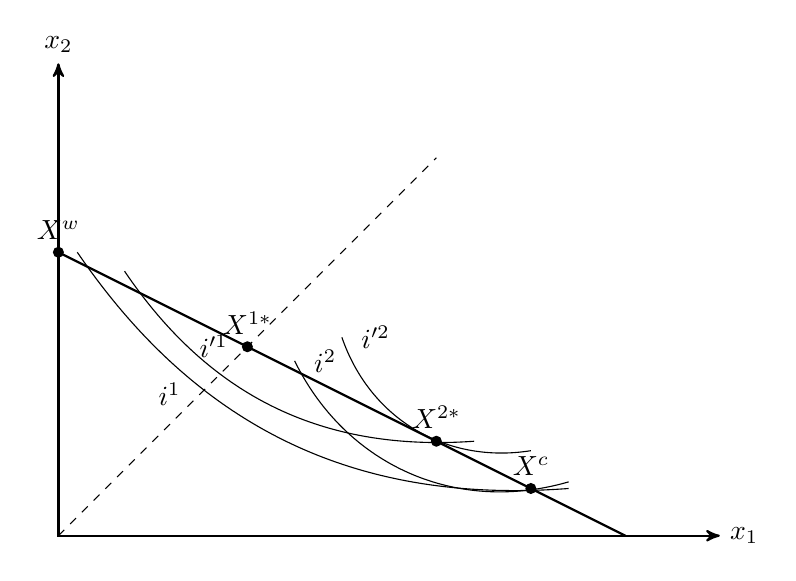
\begin{tikzpicture}[
        scale=1.2,
        IS/.style={black, thick},
        LM/.style={black, dashed},
        i1/.style={black, thin},
        i2/.style={black},
        axis/.style={thick, ->, >=stealth', line join=miter},
        every node/.style={color=black},
        dot/.style={circle,fill=black,minimum size=4pt,inner sep=0pt,
            outer sep=-1pt},
    ]
    % axis
    \draw[axis,<->] (7,0) node(xline)[right] {$x_1$} -|
                    (0,5) node(yline)[above] {$x_2$};
    \draw[IS] (0,3) coordinate (IS_1) -- (6,0) coordinate (IS_2) ;
    \draw[LM] (0,0) coordinate (IS_1) -- (4,4) coordinate (IS_2) ;
    \draw[i1] (0.2,3) to [bend right=30] coordinate[pos=0.1] (l_i) (5.4,0.5) ;
    \draw[i1] (0.7,2.8) to [bend right=30] coordinate[pos=0.1] (l_i) (4.4,1) ;
    \draw[i2] (2.5,1.85) to [bend right=40] coordinate[pos=0.1] (l_i) (5.4,0.57) ;
    \draw[i2] (3,2.1) to [bend right=40] coordinate[pos=0.1] (l_i) (5,0.9) ;
    %Intersection is calculated "manually" since Tikz does not offer
    %intersection calculation for parabolas
    \node[label=left:$i^1$] at (1.5,1.5) (int1) {};
    \node[label=left:$i'^1$] at (2,2) (int1) {};
    \node[label=right:$i^2$] at (2.5,1.85) (int1) {};
    \node[label=right:$i'^2$] at (3,2.1) (int1) {};
    
    \node[dot,label=above:$X^{1*}$] at (2,2) (int1) {};
    \node[dot,label=above:$X^{2*}$] at (4,1) (int1) {};
    \node[dot,label=above:$X^{c}$] at (5,0.5) (int1) {};
    \node[dot,label=above:$X^w$] at (0,3) (int1) {};    
\end{tikzpicture}
\end{center}
\end{figure}

We prove that we can generalize this example: a collective choice $X^c$ is Pareto efficiency if and only if it is between $X^{1*}(p,\alpha_1,\rho_1)$ and  $X^{2*}(p,\alpha_2,\rho_2)$ if both individuals' utility functions satisfy monotonicity\footnote{A utility function is \textbf{monotone} if $(x_1,x_2)>(x'_1,x'_2)$ elementwise, then $U(x_1,x_2)\geq U(x'_1,x'_2)$.} and symmetry\footnote{A utility function is \textbf{symmetric} if $U(x_1,x_2) = U(x_2,x_1)$ holds. Note that every utility function which has the form of equation (1) is symmetric in our experimental design because two states have the same chance to be chosen.}. A detailed steps are given in the appendix, but the result itself is very intuitive: a collective decision which is a compromise of group member's wants is Pareto efficient. Upon this definition, we can test Pareto efficiency for all 18 group choices.

However, even though this test is simple and easy to compute, it doesn't discriminate the severity of inefficiency. The inefficiency markedly varies across choices; some are ignorable while others are significant. To consider this, we has devised a continuous scale on the inefficiency. By construction, this index takes 0 if an observed choice is Pareto efficient. However, if a choice is inefficient, it means there exists a Pareto improvement of it. Finding a Pareto improvement choice which is closest (in euclidean distance) to the original collective choice, we measure the difference of utility at the improvement and the observed one. To adjust the scale, we normalize it with the difference of utility at the improvement and the worst case on the budget line. As this inefficiency is not same for individual 1 and 2, we take the mean of two partners. And finally, we compute the average loss across 18 times of group decisions. The index is represented as in equation (6).
   
\begin{equation}
L=\frac{1}{18}\Sigma_{j=1}^{18} \frac{1}{2}\Sigma_{i=1}^2 \frac{u_i(X^{'j})-u_i(X^{cj})}{u_i(X^{'j})-u_i(X^{wji})}
\end{equation}   

where

\begin{equation}
X^{'j}=
\begin{cases}
argmin|X^{j}-X^c| \, \textnormal{s.t.} p_jX^{j}\leq1, u_i(X^{j})\geq(>\textnormal{for some $i$}) u_i(X^c) \forall i=1,2 \\
X^c \, \textnormal{if $X^c$ is Pareto efficient} 
\end{cases}
\end{equation}

In equation (6) and (7), $u_i()$ is the estimated utility function of member $i$ from individual decisions. $X^{cj}$, and $X^{wji}$\footnote{It takes two values: spending all in more expensive goods $(x_{min},x_{max}=(0,\frac{1}{p_{expensive}})$ or the middle point of the budget line $(\frac{1}{p_1+p_2},\frac{1}{p_1+p_2})$. It depends on individual's estimated $\alpha$ and $\rho$. Whenever $\alpha\geq0.5$, the former is the worst choice. On the other hand, if $\alpha<0.5$, which means one puts more weight on maximum point $x_{max}=max(x_1,x_2)$, the latter can be worst depending on $\rho$. Out of 17730 collective decisions of 985 individuals whose CCEI is equal to or grater than 0.9, 1639 (9.2\%) are cases where the middle point is the worst group choice. For the rest, $(x_{min},x_{max}=(0,\frac{1}{p_{expensive}})$ is the most unfavorable.} indicate observed group choice and the worst case for individuals on the budget line j. In the graphical example in figure 3, $X^{'j}$ equals to individual 2's optimal choice $X^{2*}$ while both $X^{wi}$s are the intercept of $x_2$ axis. The loss index $L$ can take the value between 0 and 1. Especially, 0 means all of the group's decisions are Pareto efficient. On the other extreme, 1 denotes the group makes the worst choice all the time. $L$ between the two has the meaning of between the two, higher numbers showing more inefficiency.   

\subsection{Group Choices' Inefficiency}

Figure 8 shows the distribution of group inefficiency defined in equation (6)-(7). About 41.88\% of pairs (N=134 out of 320) have inefficiency below 0.05. Among them, only 12 groups made Pareto efficient choices every round, and other 122 groups trembled but most at unremarkable degree, which might have not been captured if we use a discrete measure. However, 28 collectives out of 320 have significant inefficiency over 0.3, showing that they have wasted a lot of resources, leaving a room for the improvement. Remaining 158 pairs have moderate inefficiency between 0.05 and 0.3.

Interestingly, there exists a strong relationship between collective rationality and group choices' inefficiency as presented in Figure 9. Specifically, the distribution of inefficiency of groups' of which collective CCEI over 0.9 first-order stochastically dominates that of groups under 0.9. As only groups with both members' individual CCEIs are over 0.9 are included in testing Pareto efficiency, in our terminology, we can also say that Pareto efficiency is positively correlated to the extension of rationality.

Note that is possible for group decision which is consistent with GARP to be Pareto inefficient. As CCEI scores internal consistency of group choices irrespective of individuals' preferences, a group can also attain high CCEI by making choices as if a third part who has a totally different preference to both individuals' stands in even though this is unnatural. 

However, the result says such unnatural scheme rarely occurs. Rather, it shows pairs selecting a consumption bundle which is a compromise of both members' wants do better in terms of unity within collective choices. 

-other factors

\end{document}